\documentclass{beamer}

\mode<presentation> {

\usetheme{default}
%\usetheme{Rochester}
%\usecolortheme{lily}

\setbeamertemplate{footline}[page number] 
\beamertemplatenavigationsymbolsempty
\setbeamertemplate{bibliography item}{} %Remove icons in bibliography
}

\usepackage{graphicx} % Allows including images
\usepackage{amsmath}
\usepackage{lmodern}
\usepackage{listings}
\usepackage{hyperref}
\usepackage{wrapfig}



\usepackage{tikz}
\usetikzlibrary{bayesnet}

\lstset{
    language=[5.0]Lua,
    basicstyle=\fontsize{11}{9},
    sensitive=true,
    breaklines=true,
    tabsize=2
}

%----------------------------------------------------------------------------------------
%	TITLE PAGE
%----------------------------------------------------------------------------------------

\title[DEF]{Topic Modelling: Deep Exponential Families} 
\subtitle{relation to SGVB}

\author{Otto Fabius} 
\institute[UvA] 
{University of Amsterdam \\
Supervisor: P.Putzky \\ 
Co-Supervisors: M. Welling, D.P. Kingma
\medskip
}
\date{\today} % Date, can be changed to a custom date

\begin{document}

\begin{frame}
\titlepage % Print the title page as the first slide
\end{frame}


%----------------------------------------------------------------------------------------
%	PRESENTATION SLIDES
%----------------------------------------------------------------------------------------

\begin{frame}
\frametitle{Intro}
\begin{itemize}
\item{Thesis on topic modelling with SGVB}
\item{Deep Exponential Families\footnote{Ranganath, Rajesh, et al. "Deep exponential families." (2014).} also performs inference over topics, with good results}
\item{What can we learn from their approach?}
\end{itemize}

\end{frame}

\section{Deep Exponential Families}

\begin{frame}
\frametitle{Deep Exponential Families (DEF)}
\begin{itemize}
\item{Idea: generative model with hierarchical latent representations.}
\item{Each layer is an exponential family (e.g. Sparse Gamma, Bernoulli, Poisson)}
\item{Natural parameters of each layer of latent variables $\mathbf{z_l}$ are controlled by inner product of previous layer $\mathbf{z_{l-1}}$ and learned weights $\mathbf{w_l}$}
\item{Perform inference with "black box variational inference"\footnote{Ranganath, Rajesh, Sean Gerrish, and David M. Blei. "Black Box Variational Inference." (2013).}, using a mean field approximation family as inference model $q$}
\end{itemize}
\end{frame}

\begin{frame}
\frametitle{Deep Exponential Families (DEF)}
\begin{figure}
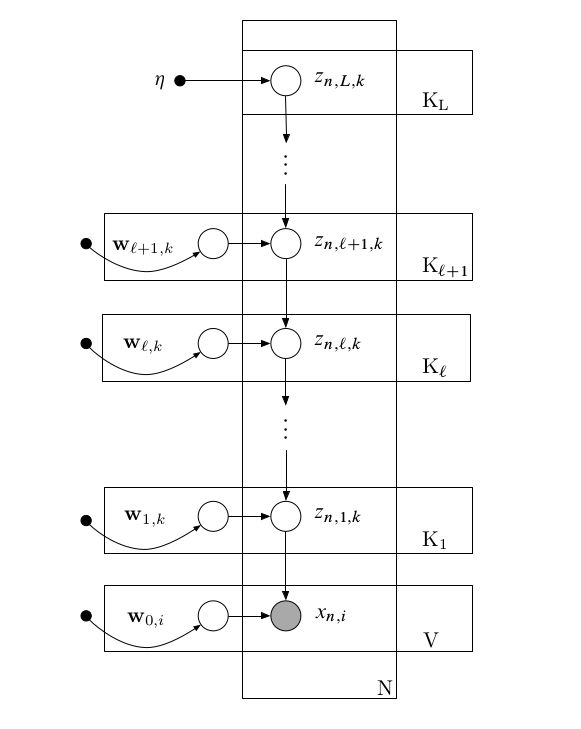
\includegraphics[scale=0.3]{DEF_structure.png}
\end{figure}
\end{frame}

\begin{frame}
\frametitle{Black Box Variational Inference}
Using a simple approximation q from the mean field variational family, optimize lower bound: 
\begin{figure}
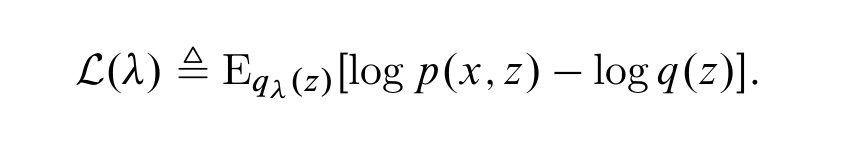
\includegraphics[scale=0.3]{ELBO.png}
\end{figure}
Sampling $z \sim q_\lambda (z)$ to obtain gradients, using some variance reduction techniques.
\end{frame}



\begin{frame}{}
\frametitle{LDA and SGVB Topic Model}
\begin{minipage}[r]{0.45\textwidth}
\centering
    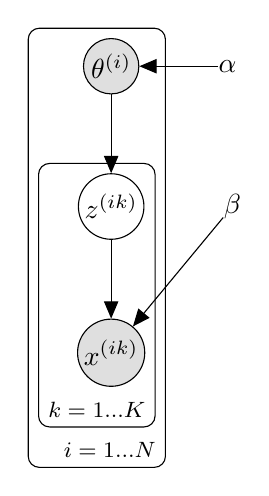
\begin{tikzpicture}[node distance = 1.5cm]
        \node[obs] (x) {$x^{(ik)}$}; 

        \node[latent, above=of x] (z) {$z^{(ik)}$}; 
        
        \node[obs, above=of z] (d) {$\theta^{(i)}$}; 

        \node[const, right=of d] (a) {$\alpha$} ;
        \node[const, right=of z] (th) {$\beta$} ;
		
		\edge {a} {d};
        \edge {z} {x};
        \edge {d} {z};
        \edge {th} {x};

		
		\plate {xz} {(x)(z)} {$k = 1...K$};
        \plate {xzd} {(x)(z)(d)(xz)} {$i = 1...N$};
	  
    \end{tikzpicture}
\end{minipage}%
\begin{minipage}{0.50\textwidth}
    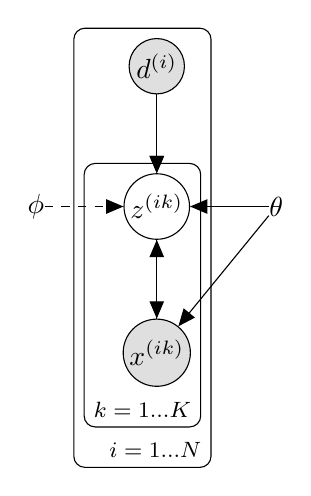
\begin{tikzpicture}[node distance = 1.5cm]
        \node[obs] (x) {$x^{(ik)}$}; 

        \node[latent, above=of x] (z) {$z^{(ik)}$}; 
        
        \node[obs, above=of z] (d) {$d^{(i)}$}; 

        \node[const, right=of z] (th) {$\theta$} ;
        \node[const, left=of z] (ph) {$\phi$};

        \edge {z} {x};
        \edge {d} {z};
        \edge {th} {z};
        \edge {th} {x};

        \edge [dashed] {ph} {z}
        \edge [dashed,bend right] {d} {z}
        \edge [dashed,bend left] {x} {z}
		
		\plate {xz} {(x)(z)} {$k = 1...K$};
        \plate {xzd} {(x)(z)(d)(xz)} {$i = 1...N$};

    \end{tikzpicture}
\end{minipage}

\vspace{5mm}

\hspace{15mm} LDA \hspace{25mm} SGVB Topic Model
\end{frame}

\begin{frame}
\frametitle{Why use SGVB?}
\begin{itemize}
\item{Inference is faster with SGVB than with BBVI\footnote{I don't have proof or an explicit comparison of the methods}, especially in larger/deeper models}
\item{SGVB had a more powerful inference model that also scales well with many documents: DEF uses seperate parameters for the inference model $q$ for each document!}
\end{itemize}
\end{frame}

\begin{frame}
\frametitle{What can we learn from DEF?}
\begin{itemize}
\item{Using a hierarchical structure for Bag-Of-Words topic modelling is a good idea.}
\item{As opposed to in LDA, a powerful generative model does not necessarily need to generate separate words. Instead, it can generate documents (word count vectors)}
\end{itemize}
\end{frame}

\begin{frame}
\frametitle{Miscellaneous thoughts}
\begin{itemize}
\item{DEF uses multiple (stochastic) latent variables. This means one can easily inspect the latent representations of a document for each level. Not clear what hidden layer activations of an MLP would represent. Other possible advantages of multiple layers of latent variables?}
\item{What is the best choice for output distribution of word counts? (Poisson? Beta-Binomial (constrained or unconstrained)?)}
\end{itemize}
\end{frame}



\end{document}